% !TEX root = 15cvpr.tex
\section{Introduction}

\begin{figure}[t]
\begin{center}
    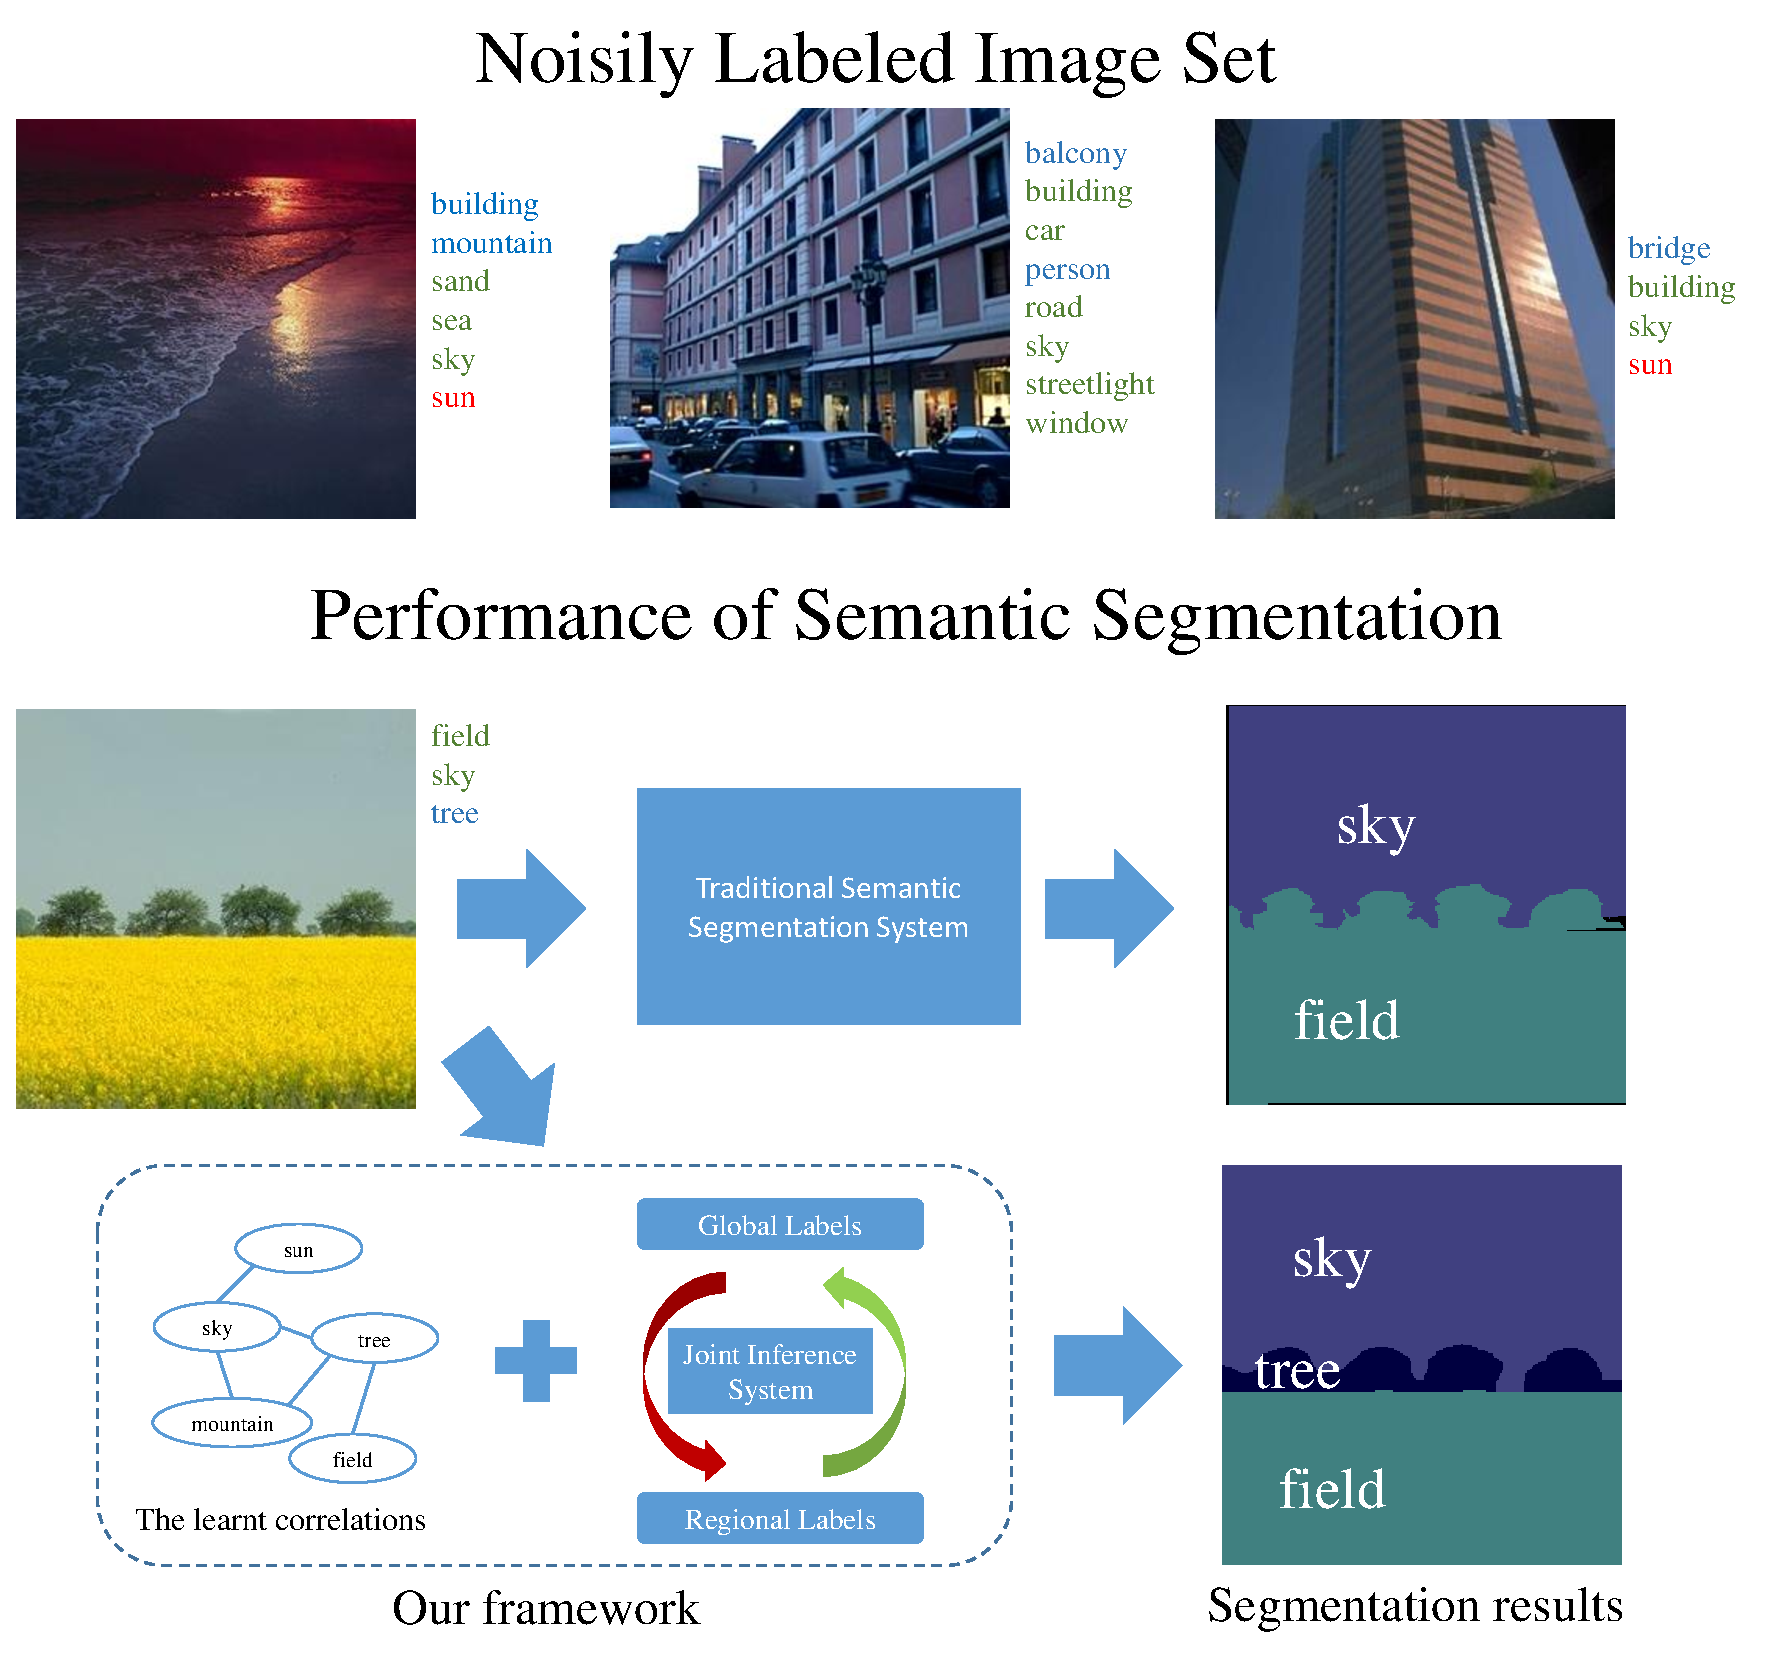
\includegraphics[width=1\linewidth]{fig_noisyparsing.pdf}
\end{center}
    \caption{Given a set of social images and their associated labels where label may be precise (green), incorrect (red) or missing (blue), we learn a model that segments and recognizes visual concept in images. Best viewed in color.}
\label{fig:noisyparsing}
\vspace{-3mm}
\end{figure}

Semantic segmentation, \ie, parsing image into several semantic regions, assigns each pixel (or superpixel) to one of the predefined semantic categories.
Most state-of-the-art approaches heavily rely on a sufficiently huge amount of annotated samples in training.
However, there are no enough labeled samples for this task because pixel-level (or superpixel-level) annotation is time-consuming and labor-intensive.
Recent works have begun to address the semantic segmentation problem in the weakly supervised settings, where each training image is annotated by image-level labels but no pixel-level annotation is given \cite{verbeek2007region,vezhnevets2010towards,vezhnevets2011weakly,vezhnevets2012weakly,xu2014tell,zhang2013sparse,zhang2013probabilistic}.
The existing weakly supervised semantic segmentation methods are based on an unrealistic assumption that image-level labels are provided by professional annotators, and thus are correct and complete.


With the prevalence of photo sharing websites and collaborative image tagging system, such as Flickr, a large number of social images with user provided labels are available from the Internet.
These labels are usually image-level; moreover, the quality of labels is not satisfactory: they are often imprecise and incomplete!
Figure \ref{fig:noisyparsing} illustrates a set of representative social images and its associated labels.
We can observe that only limited labels accurately describe the visual content of the image, while other labels are imprecise.
Moreover, some important labels, which are highly associated with the image, are missing.
It is challenging but attractive to learn an effective semantic segmentation model from such social images.

In this paper, we present a weakly supervised method that, for the first time, overcomes the challenge posed by noisy annotations.
The proposed method learns a joint conditional random field (CRF) model from weakly labeled social images by sufficiently leveraging various contexts, \eg, the associations between high-level semantic concepts and low-level visual appearance, inter-label correlations, spatial neighborhood cues, and the label consistency between image-level and pixel-level.
More specifically, we extract global features for the whole image and local features for the superpixels in multiple scales by convolutional neural network (CNN) and latent semantic concept model (LSC).
Then we capture the inter-label correlations by visual contextual cues as well as label co-occurrence statistics.
The label consistency between image-level and pixel-level is finally achieved by iterative refinement in a flip-flop manner.

To illustrate both robustness and effectiveness of our method, we demonstrate experimental results on two challenging datasets, PASCAL VOC 2007 and SIFT-flow datasets, which are representative of the hardness of annotation noise occurred in social images.
Our method outperforms previous state-of-the-art approaches on standard datasets, demonstrating that the image-level annotation, especially potential relationships, is more efficiently utilized by our method.

The main contributions of this paper are summarized as follows:
\begin{itemize}
  \item We propose a weakly supervised semantic segmentation model for social images, where only image-level labels are available for training, or even worse, the annotations can be imprecise or incomplete.
  \item We design a joint learning framework to sufficiently leverage various contexts including feature-label association, inter-label correlation, and spatial neighborhood cues.
  \item We explore an effective strategy that cooperatively captures label co-occurrence statistics as well as visual contextual cues to model the label correlations, in addition to refine noisy labels.
\end{itemize}
